\documentclass[12pt]{article}
\usepackage[paper=letterpaper,margin=1.5cm]{geometry}
\usepackage{amsmath}
\usepackage{amssymb}
\usepackage{amsfonts}
\usepackage{mathtools}
%\usepackage[utf8]{inputenc}
%\usepackage{newtxtext, newtxmath}
\usepackage{lmodern}     % set math font to Latin modern math
\usepackage[T1]{fontenc}
\renewcommand\rmdefault{ptm}
%\usepackage{enumitem}
\usepackage[shortlabels]{enumitem}
\usepackage{titling}
\usepackage{graphicx}
\usepackage[colorlinks=true]{hyperref}
\usepackage{setspace}
\usepackage{subfigure} 
\usepackage{braket}
\usepackage{color}
\usepackage{tabularx}
\usepackage[table]{xcolor}
\usepackage{listings}
\usepackage{mathrsfs}
\usepackage{stackengine}
\usepackage{physics}
\usepackage{afterpage}
\usepackage{pdfpages}
\usepackage[export]{adjustbox}
\usepackage{biblatex}

\setstackEOL{\\}

\definecolor{dkgreen}{rgb}{0,0.6,0}
\definecolor{gray}{rgb}{0.5,0.5,0.5}
\definecolor{mauve}{rgb}{0.58,0,0.82}


\lstset{frame=tb,
  language=Python,
  aboveskip=3mm,
  belowskip=3mm,
  showstringspaces=false,
  columns=flexible,
  basicstyle={\small\ttfamily},
  numbers=none,
  numberstyle=\tiny\color{gray},
  keywordstyle=\color{blue},
  commentstyle=\color{dkgreen},
  stringstyle=\color{mauve},
  breaklines=true,
  breakatwhitespace=true,
  tabsize=3
}
\setlength{\droptitle}{-6em}

\makeatletter
% we use \prefix@<level> only if it is defined
\renewcommand{\@seccntformat}[1]{%
  \ifcsname prefix@#1\endcsname
    \csname prefix@#1\endcsname
  \else
    \csname the#1\endcsname\quad
  \fi}
% define \prefix@section
\newcommand\prefix@section{}
\newcommand{\prefix@subsection}{}
\newcommand{\prefix@subsubsection}{}
\renewcommand{\thesubsection}{\arabic{subsection}}
\makeatother
\DeclareMathOperator*{\argmin}{argmin}
\newcommand{\partbreak}{\begin{center}\rule{17.5cm}{2pt}\end{center}}
\newcommand{\alignbreak}{\begin{center}\rule{15cm}{1pt}\end{center}}
\newcommand{\tightalignbreak}{\vspace{-5mm}\alignbreak\vspace{-5mm}}
\newcommand{\hop}{\vspace{1mm}}
\newcommand{\jump}{\vspace{5mm}}
\newcommand{\R}{\mathbb{R}}
\newcommand{\C}{\mathbb{C}}
\newcommand{\N}{\mathbb{N}}
\newcommand{\G}{\mathbb{G}}
\renewcommand{\S}{\mathbb{S}}
\newcommand{\bt}{\textbf}
\newcommand{\xdot}{\dot{x}}
\renewcommand{\star}{^{*}}
\newcommand{\ydot}{\dot{y}}
\newcommand{\lm}{\mathrm{\lambda}}
\renewcommand{\th}{\theta}
\newcommand{\id}{\mathbb{I}}
\newcommand{\si}{\Sigma}
\newcommand{\Si}{\si}
\newcommand{\inv}{^{-1}}
\newcommand{\T}{^\intercal}
\renewcommand{\tr}{\text{tr}}
\newcommand{\ep}{\varepsilon}
\newcommand{\ph}{\varphi}
%\renewcomand{\norm}[1]{\left\lVert#1\right\rVert}
\definecolor{cit}{rgb}{0.05,0.2,0.45}
\addtolength{\jot}{1em}
\newcommand{\solution}[1]{

\noindent{\color{cit}\textbf{Solution:} #1}}

\newcounter{tmpctr}
\newcommand\fancyRoman[1]{%
  \setcounter{tmpctr}{#1}%
  \setbox0=\hbox{\kern0.3pt\textsf{\Roman{tmpctr}}}%
  \setstackgap{S}{-.9pt}%
  \Shortstack{\rule{\dimexpr\wd0+.1ex}{.9pt}\\\copy0\\
              \rule{\dimexpr\wd0+.1ex}{.9pt}}%
}

\newcommand{\Id}{\fancyRoman{2}}

% Enter the specific assignment number and topic of that assignment below, and replace "Your Name" with your actual name.
\title{STAT 37710: Homework 2}
\author{Caleb Derrickson}
\date{April 17, 2024}

\begin{document}
\onehalfspacing
\maketitle
\allowdisplaybreaks
{\color{cit}\vspace{2mm}\noindent\textbf{Collaborators:}} The TA's of the class, as well as Kevin Hefner, and Alexander Cram, and Alice Yang.

\tableofcontents

\newcommand{\scS}{\mathcal{S}}


\newpage
\section{Problem 1} 
Let $A$ be a symmetric $d \times d$ matrix.
\subsection{Problem 1, part a}
Show that if \textbf{v} and \textbf{v}' are two eigenvectors of $A$ with corresponding eigenvalues $\lm \neq \lm'$, then \textbf{v} is orthogonal to \textbf{v}'.
\partbreak
\begin{solution}

    We have that $A \in \R^{d\times d}$, so $A\T \in \R^{d\times d}$. Then, we have the following:
    \[(\textbf{v}')\T A \textbf{v} = (\textbf{v}')\T \textbf{v}\]
    Note that the quadratic form also has the following form
    \[(\textbf{v}')\T A \textbf{v} = (A\T\textbf{v}')\T \textbf{v} = \lm' (\textbf{v}')\T \textbf{v}.\]
    These two equations are equivalent, so we must then have 
    \[(\textbf{v}')\T \textbf{v} = \lm' (\textbf{v}')\T \textbf{v} \iff (\lm - \lm') (\textbf{v}')\T \textbf{v} = 0.\]
    Since $\lm \neq \lm'$, we have that $(\textbf{v}')\T \textbf{v} = 0$. 
\end{solution}

\newpage
\subsection{Problem 1, part b}
Show that if $\scS$ is a set of eigenvectors of $A$ with the same eigenvalue $\lm$ and $\scS$ spans a subspace $V$ of $\R^d$ of dimension $k$, then one can find $k$ mutually orthogonal vectors $\textbf{v}^1, \textbf{v}^2, ..., \textbf{v}^k$ such that (a) $V =$ span$\{ \textbf{v}^1, ..., \textbf{v}^k\}$, and (b) each $\textbf{v}^{(i)}$ is an eigenvector of $A$ with eigenvalue $\lm$. 
\partbreak
\begin{solution}

    Let $\textbf{v}_1, \textbf{v}_2, ..., \textbf{v}_k$ be the eigenvectors with same eigenvalue $\lm$. These eigenvectors are not guaranteed to by mutually orthogonal - we can however, recover a set or orthogonal vectors $\textbf{w}_1, ..., \textbf{w}_k$ via Gram Schmidt. These $\textbf{w}_i$ are a linear combination of the $\textbf{v}_i$'s , thus will have the same eigenvalue as the $\textbf{v}_i$'s. Since the $\textbf{w}_i$'s are orthogonal, we have that $V = \text{span}\{\textbf{w}_1, ..., \textbf{w}_k\}$ with dimension $k$. Therefore, a set of vectors has been found.  
\end{solution}


\newpage
\subsection{Problem 1, part c}
Explain why the above two statements imply that $A$ has an eigenvector decomposition of the form 
\[A = \sum_{i = 1}^d \lm_i \textbf{v}_i \textbf{v}_i\T,\]
where each $\textbf{v}_i$ is a unit eigenvector of $A$ and $\lm_i$ is the corresponding eigenvalue.
\partbreak
\begin{solution}
    
    Since $A$ is symmetric, all its eigenvalues are real valued. Thus, we assume we have $d$ real valued eigenvalues $\lm_i$. Note that these eigenvalues are not necessarily unique, however. To this extent, suppose we have $m$ distinct eigenvalues, each with at least one corresponding eigenvector. Suppose for $\textbf{v}_i$, we have that $A\textbf{v}_i = \lm \textbf{v}_i$. By the previous part, we saw that we could recover a set of orthogonal vectors $\textbf{w}_1, ..., \textbf{w}_k$, which I will call these $\textbf{v}_1, ..., \textbf{v}_k$ for the sake of simplicity. If we gather all eigenvectors corresponding to the same eigenvalue, say $\textbf{v}_1, ..., \textbf{v}_k$, we then have $A\textbf{v}_1 = \lm\textbf{v}_1, ..., A\textbf{v}_k = \lm \textbf{v}_k$.  Expressing these in the form of matrices, we have $AV_i = \Lambda_i V_i$, where $\Lambda_i = \lm_i\id$ and $V_i$ is the matrix whose columns are formed by the eigenvectors of $\lm_i$. Assume without loss of generality that the eigenvectors have been normalized so that $\textbf{v}_i\T \textbf{v}_j = \delta_{ij}$. This implies that $V_i\T V_i = \id$, but not necessarily that $V_iV_i\T = \id$. We will show that this is the case.

    \jump
    Suppose we have a vector $\textbf{x}$ which is a linear combination of our eigenvectors $\textbf{v}_1, ..., \textbf{v}_k$. Then we see that 
    \[V_iV_i\T \textbf{x}= \left(\sum_{i = 1}^k \textbf{v}_i\textbf{v}_i\T \right)\sum_{i = 1}^k \alpha_i\textbf{v}_i = \sum_{i = 1}^k \textbf{v}_i\textbf{v}_i\T (\alpha_i \textbf{v}_i) + 0 = \sum_{i = 1}^k \alpha_i \textbf{v}_i = \textbf{x}.\]
    Note the cross terms in the third expression cancel out, since the eigenvectors are orthogonal. Therefore, the matrix $V_iV_i\T$ acts like the identity matrix of size $k$ for vectors which span the given eigenvectors. Therefore, 
    \[AV_i = \Lambda_i V_i \iff A = AV_iV_i\T = V_i\Lambda V_i\T = \sum_{j = 1}^k \lm_i \textbf{v}_j^{(i)} (\textbf{v}_j^{(i)})\T\]
    This isn't \textit{necessarily} true, however, since the dimensions don't match up. This is no problem, since we can simply sum over all subspaces $V_i$. Since we said that there will be $m$ distinct eigenvalues, we have $m$ distinct subspaces, which we are summing over. Therefore, we have that 
    \[A = \sum_{i = 1}^d \lm_i \textbf{v}_i \textbf{v}_i\T,\]
    since eigenvectors corresponding to difference eigenvalues are inherently orthogonal. Therefore, the statement has been shown. 
    
\end{solution}

\newpage
\subsection{Problem 1, part d}
Assume that $\lm_1 \leq \lm_2 \leq ... \leq \lm_d$. Show that 
\[\argmin_{\textbf{w} \in \R^d \setminus \{0\}} \frac{\textbf{w}\T A\textbf{w}}{\norm{\textbf{w}}^2} = \textbf{v}_1 \quad \text{and} \quad \argmax_{\textbf{w} \in \R^d \setminus \{0\}}  \frac{\textbf{w}\T A\textbf{w}}{\norm{\textbf{w}}^2} = \textbf{v}_d.\]
\partbreak
\begin{solution}

    Suppose we have that $\textbf{w}$ is a linear combination of the eigenvectors of $A$. That is, $\textbf{w} = \sum_{i =1}^d \alpha_i \textbf{v}_i$. Then, we have
    \[\textbf{w}\T A\textbf{w} = \textbf{w}\T \left (\sum_{i = 1}^d \alpha_i \lm_i \textbf{v}_i\right) = \sum_{i  =1}^d \alpha_i^2 \lm_i.\]
    By the definition of the two norm on $\R^d$, the inner product of $\textbf{w}$ with itself is its norm squared. Therefore, $\norm{\textbf{w}}^2 = \braket{\textbf{w}}{\textbf{w}} = \sum_{i = 1}^d \alpha_i^2$. Therefore, the given ratios are of the form, 
    \[\frac{\textbf{w}\T A\textbf{w}}{\norm{\textbf{w}}^2} = \frac{\sum_{i = 1}^d \alpha_i^2 \lm_i}{\sum_{i = 1}^d \alpha_i^2}.\]
    Suppose that $\lm_j$ is the smallest eigenvalue of $A$. Certainly, this implies 
    \[\frac{\textbf{w}\T A\textbf{w}}{\norm{\textbf{w}}^2} = \frac{\sum_{i = 1}^d \alpha_i^2 \lm_i}{\sum_{i = 1}^d \alpha_i^2} \geq \frac{\lm_j\sum_{i = 1}^d \alpha_i^2 }{\sum_{i = 1}^d \alpha_i^2} = \lm_j.\]
    This bound is achievable only when $\textbf{w}$ is a multiple of only the eigenvector corresponding to $\lm_j$, which I will denote as $\textbf{v}_j$. Aside from $\textbf{w}$ being the zero vector, this is the lowest bound achievable by any $\textbf{w}$ in the span of $A$, since if there were, then $\lm_j$ wouldn't be the smallest eigenvalue. Therefore, the first equality has been shown. The second one can be similarly shown with instead utilizing the largest eigenvalue of $A$, giving us an achievable upper bound. 


\end{solution}

\newpage
\section{Problem 2}
Let $\{\textbf{x}_1, ..., \textbf{x}_n\}$ be a dataset of $n$ vectors in $\R^d$ that have already been centered, i.e., $\sum_{i = 1}^n \textbf{x}_i = 0$. Let $\textbf{p}_1, ..., \textbf{p}_k$ be a set of $k$ mutually orthogonal unit vectors, and $V$ the subspace that they span. 
\subsection{Problem 2, part a}
Given any $\textbf{x} \in \R^d$, let $\textbf{x}_V$ be the closest point to \textbf{x} in $V$, i.e., $\textbf{x}_V = \argmin_{\textbf{y} \in V}\norm{\textbf{x} - \textbf{y}}^2$. Show that $\textbf{x}_V$ is given by the orthogonal projection of \textbf{x} to $V$, i.e.,
\[\textbf{x}_V = \sum_{i = 1}^k (\textbf{x}\cdot \textbf{p}_i) \textbf{p}_i.\]
\partbreak
\begin{solution}

    Denote the projection $P : \R^d \to \R^d$ which projects any vector $\textbf{x}\in \R^d$ to $V$. Define $P$ as $P = \sum_{i = 1}^k \textbf{p}_i \textbf{p}_i\T.$\footnote{This is clearly well defined.} This is equivalent to saying that $P\textbf{x} = \textbf{x}_V$ \textit{in spirit} - to show that $P\textbf{x}$ is of the given form, we need to do some work. First, we will show that $\textbf{x} - P\textbf{x} \in V^\perp$. This is straightforward, since for any $\textbf{p}_j$, we have that 
    \[\left(\textbf{x} - P\textbf{x}\right)\T \textbf{p}_j = \textbf{x}\T \textbf{p}_j - \left( \sum_{i = 1}^d (\textbf{x}\T \textbf{p}_i) \textbf{p}_i\right)\T \textbf{p}_j = \textbf{x}\T \textbf{p}_i - (\textbf{x}\T\textbf{p}_i)(\textbf{p}_i\T\textbf{p}_i) = 0.\]
    Since $V$ is a linear subspace, then for any $\textbf{y} \in V$, $P\textbf{x} - \textbf{y} \in V$. Therefore, the following can be shown: for any $\textbf{y} \in V$,
    \begin{align*}
        \norm{\textbf{x} - \textbf{y}}^2 &= \norm{\textbf{x} - P\textbf{x} + P\textbf{x} - \textbf{y}}^2\\
        &=\left( \textbf{x} - P\textbf{x} + P\textbf{x} - \textbf{y}\right)\T\left(\textbf{x} - P\textbf{x} + P\textbf{x} - \textbf{y}\right)\\
        &= \norm{\textbf{x} - P\textbf{x}}^2 + \norm{P\textbf{x} - \textbf{y}}^2 + 2\left(\textbf{x} - P\textbf{x}\right)\T\left(P\textbf{x} - \textbf{y}\right). 
    \end{align*}

    What I did above was simple expansion. Since $\textbf{x} - P\textbf{x} \in V^\perp$, and $P\textbf{x} - \textbf{y} \in V$, then their inner product is zero by definition. The equation above results in $\norm{\textbf{x} - \textbf{y}}^2 = \norm{\textbf{x} - P\textbf{x}}^2 + \norm{P\textbf{x} - \textbf{y}}^2$. \footnote{This is pretty much the Pythagorean theorem.} This can be bounded below by $\norm{\textbf{x} - P\textbf{x}}^2$, which can be achieved by setting $y = P\textbf{x}$. This is then the minimum of the function, since the second term is $\geq 0$, and only zero when its argument is zero. Therefore, $P\textbf{x} = \textbf{x}_V$. Note by the given form of the projection, we have 
    \[P\textbf{x} = \sum_{i = 1}^k \textbf{p}_i\textbf{p}_i\T \textbf{x} = \sum_{i = 1}^k (\textbf{p}_i \cdot \textbf{x})\textbf{p}_i = \textbf{x}_V.\]
    
\end{solution}

\newpage
\subsection{Problem 2, part b}
Let $\Phi(V)$ be the mean squared error of projecting $\{\textbf{x}_1, ..., \textbf{x}_n\}$ to $V$,
\[\Phi(V) = \frac{1}{n}\sum_{i = 1}^n \norm{\textbf{x}_i - (\textbf{x}_i)_{V}}^2.\]
Show that $\Phi(V)$ is minimized by setting $\textbf{p}_1, ..., \textbf{p}_k$ to be the $k$ leading eigenvectors of the sample covariance matrix $\hat{\Sigma} = \frac{1}{n}\sum_{i = 1}^n \textbf{x}_i \textbf{x}_i\T.$
\partbreak
\begin{solution}

    We will go straight into calculations.
    \tightalignbreak
    \begin{align*}
        &\argmin \Phi(V) = \argmin \frac{1}{n}\sum_{i  =1}^n\norm{\textbf{x}_i - (\textbf{x}_i)_V}^2 &\text{(Given.)}\\
        &= \argmin \frac{1}{n} \sum_{i = 1}^n\norm{\textbf{x}_i - \sum_{j = 1}^k (\textbf{x}_i\T \textbf{p}_j)\textbf{p}_j}^2 &\text{(Last part.)}\\
        &= \argmin \frac{1}{n} \sum_{i  =1}^n\left[ \textbf{x}_i\T\textbf{x}_i - 2\textbf{x}_j\T \sum_{j = 1}^k (\textbf{x}_i\T \textbf{p}_j) \textbf{p}_j + \sum_{j = 1}^k (\textbf{x}_i\T \textbf{p}_j)^2\right] &\text{(Expanding.)}\\
        &= \argmin \frac{1}{n} \sum_{i = 1}^n\sum_{j = 1}^k -(\textbf{x}_i\T\textbf{p}_j)^2 &\text{(Simplifying.)}\\
        &= \argmax \frac{1}{n}\sum_{i = 1}^n \sum_{j = 1}^k (\textbf{x}_i\T \textbf{p}_j)^2 &\text{(Flipping signs.)}\\
        &= \argmax \frac{1}{n}\sum_{i = 1}^n\sum_{j = 1}^k \textbf{p}_j\T(\textbf{x}_i\textbf{x}_i\T)\textbf{p}_j &\text{(Associativity.)}\\
        &= \argmax \sum_{j  =1}^k \textbf{p}_j\T \left(\frac{1}{n}\sum_{i = 1}^n \textbf{x}_i \textbf{x}_i\T \right)\textbf{p}_j &\text{(Rearranging.)}\\
        &= \argmax \sum_{j = 1}^k \textbf{p}_j\T \hat{\Sigma}\textbf{p}_j &\text{(Given.)}
    \end{align*}
    \vspace{-12mm}\alignbreak
    Supposing that all $\textbf{p}_j$'s are unique, in order to maximize this function, we just take $\textbf{p}_1$, ..., $\textbf{p}_k$ to be the $k$ largest eigenvectors of $\hat{\Sigma}$. This is fine to do, since the covariance matrix is symmetric, so our work in problem 1 is applicable. 
\end{solution}

\newpage
\section{Problem 3}
Let $K$ be the Gram matrix of $n$ points in $\R^d$ (with $n \geq d$).
\newcommand{\hpipe}{\rule[0.5ex]{1.25em}{0.5pt}}
\subsection{Problem 3, part a}
Show that $\rank(K) \leq d$.
\partbreak
\begin{solution}

    This can be seen via a reinterpretation of matrix multiplication. Suppose we have the matrices $A$ and $B$, where $A$ has rows of the given $\textbf{x}$, and $B$ has columns of the given $\textbf{x}$. Their product is then given as
    \[AB = \mqty[\hpipe&\textbf{x}_1&\hpipe\\&\vdots&\\\hpipe&\textbf{x}_n&\hpipe]\mqty[|&&|\\\textbf{x}_1&...&\textbf{x}_n\\|&&|] = \mqty[\textbf{x}_1\T \textbf{x}_1 &...&\textbf{x}_1\T \textbf{x}_n\\&|&\\\textbf{x}_n\T\textbf{x}_1 &...&\textbf{x}_n\T \textbf{x}_n]\]
    Therefore, the product of $A$ and $B$ is equal to the Gram matrix. Let us examine the dimensions of the above matrices: we have that $A \in \R^{d \times n}$, $B \in \R^{n \times d}$, and $K \in \R^{d \times d}$. An elementary proof in Linear algebra states that 
    \[\rank(AB) \leq \min\{\rank(A), \rank(B)\}.\]
    Plugging in what we have, that is, $\rank(A) = d, \rank(B) = n$, and $n \geq d$, we have that $\rank(K) = \rank(AB) \leq d$, which is what we wanted to show.  
\end{solution}


\newpage
\subsection{Problem 3, part b}
Let $K \in \R^{n\times n}$ be a (symmetric) positive semi-definite matrix of rank $r$, and let $d \geq r$. Find $n$ points $\textbf{x}_1, ..., \textbf{x}_n \in \R^d$ such that their Gram matrix is $K$. 
\partbreak
\begin{solution}

    Since $K$ is symmetric, we have by problem 1 that $K$ can be rewritten as 
    \[K = Q\Lambda Q\T,\]
    where $Q$ is the matrix of eigenvectors of $K$, and $\Lambda$ its eigenvalues. Since $K$ is again, symmetric, all entries of the diagonal matrix are real and positive. We can then define $\Lambda^{1/2}$ such that $\Lambda^{1/2}\Lambda^{1/2} = \Lambda$. Define $\textbf{x}_i$ such that
    \[\textbf{x}_i = \left(\left[ Q\Lambda^{1/2}\right]_{i}\right)\T\]
    And define $A$ to have its columns as these $\textbf{x}_i$'s. From the previous part, we can see that $A\T = B$, therefore, 
    \[K = A B = A A\T = \left(\left[ Q\Lambda^{1/2}\right]\right)\left(\left[ Q\Lambda^{1/2}\right]\right)\T = Q\Lambda Q\T.\]
    Therefore, a matrix $A$ has been found. 
\end{solution}
\newcommand{\1}{\mathbbm{1}}

\newpage
\section{Problem 4}
Define the $n$ dimensional centering matrix $P = \id - \frac{1}{n} \1 \1\T$, where $\1$ is the $n$ dimensional all ones vector. 
\subsection{Problem 4, part a}
Show that $P$ is a projection operator, i.e., that $P^2 = P$.
\partbreak
\begin{solution}

    We will go straight into calculations. Note the difference between the characters $\id$ and $\1$. I wanted to use $\1$ since it looks cool. 
    \tightalignbreak
    \begin{align*}
        &P^2 = (\id - \frac{1}{n}\1\1\T)(\id - \frac{1}{n}\1\1\T) &\text{(Given.)}\\
        &= \id - \frac{2}{n}\1\1\T + \frac{1}{n^2} \1\1\T\1\1^T &\text{(Expanding.)}\\
        &= \id - \frac{2}{n}\1\1\T + \frac{1}{n}\1\1\T &(\1\T\1 = n.)\\
        &= \id - \frac{1}{n}\1\1\T &\text{(Simplifying.)}\\
        &= P &\text{(Given.)}
    \end{align*}\vspace{-12mm}\alignbreak
\end{solution}


\newpage
\subsection{Problem 4, part b}
Show that the kernel of $P$ is the line $U = \{\lm\1\}$, i.e., $P\textbf{v} = 0$ if and only if $\textbf{v} \in U$ or $\textbf{v} = 0$.
\partbreak
\begin{solution}

    If $\textbf{v} = 0$, then it is easy to see that $P\textbf{v}= 0$, since $P$ is a linear operator. We then assume that $\textbf{v} \neq 0$. Then 
    \[P\textbf{v} = \textbf{v} - \frac{1}{n}\1\1\T\textbf{x} = 0 \implies \textbf{x} = \left(\frac{\1\T \textbf{x}}{n}\right) \1 = \Bar{\textbf{x}}\1\]
    where $\Bar{\textbf{x}}$ is the average value of $\textbf{x}$. Therefore, the kernel of $P$ is shown to be the following form. 
\end{solution}


\newcommand{\bmu}{\boldsymbol{\mu}}
\newpage
\subsection{Problem 4, part c}
Let $\{ \textbf{x}_1, ..., \textbf{x}_n\}$ be a set of $n$ points in $\R^d$, and let $\Tilde{G}$ be their centered Gram matrix, $\Tilde{G}_{i, j} = (\textbf{x}_i - \bmu)\T (\textbf{x}_j - \bmu)$, where $\bmu = \frac{1}{n}\sum_{i = 1}^n \textbf{x}_i$. Show that
\[\Tilde{G} = -\frac{1}{2}PDP,\]
where $D_{i, j} = \norm{\textbf{x}_i - \textbf{x}_j}^2.$
\partbreak
\begin{solution}

    For the sake of analysis, I will show that $-2\Tilde{G} = PDP$. We then have the following:
    \tightalignbreak
    \begin{align*}
        &PDP = \left(\id - \frac{1}{n}\1\1\T\right)D\left(\id - \frac{1}{n}\1\1\T\right) &\text{(Given.)}\\
        &= D - \frac{1}{n}\1\1\T D - \frac{1}{n}D\1\1\T + \frac{1}{n^2}\1\1\T D\1\1\T &\text{(Expanding.)} \\
        \implies &\left[PDP\right]_{i, j} = \left[D - \frac{1}{n}\1\1\T D - \frac{1}{n}D\1\1\T + \frac{1}{n^2}\1\1\T D\1\1\T\right]_{i, j}\\
        &= \norm{x_i - x_j}^2 - \frac{1}{n}\sum_{k = 1}^n\norm{x_k - x_j}^2 -\frac{1}{n}\sum_{k = 1}^n\norm{x_i - x_k}^2\\&\hspace{10mm} + \frac{1}{n^2}\sum_{k = 1}^n\sum_{\ell = 1}^n\norm{x_k - x_\ell}^2 &\text{(Expanding.)}\\
        &= x_i\T x_i - 2x_i\T x_j + x_j\T x_j - \frac{1}{n}\sum_{k=1}^n\left[x_k\T x_k - 2x_k\T x_j + x_j\T x_j\right] \\&\hspace{10mm}- \frac{1}{n}\sum_{k = 1}^n\left[x_i\T x_i - 2x_i\T x_k + x_k\T x_k\right] \\&\hspace{10mm}+ \frac{1}{n^2}\sum_{k = 1}^n\sum_{\ell = 1}^n\left[x_k\T x_k - 2x_k\T x_\ell + x_{\ell}\T x_{\ell}\right] &\text{(Expanding.)}\\
        &= x_i\T x_i - 2x_i\T x_j + x_j\T x_j - \left(\frac{2}{n}\sum_{k = 1}^nx_k\T x_k\right) + 2\bmu\T x_j - x_j\T x_j \\&\hspace{10mm}- x_i\T x_j + 2x_i\T \bmu + \sum_{k = 1}^n\left[\frac{x_k\T x_k}{n} - \frac{2}{n}x_k\T \bmu + \frac{1}{n^2}\sum_{\ell = 1}^n x_\ell \T x_\ell\right] &\text{(Grouping, Expanding.)}\\
        &= -2c_i\T x_j - \frac{1}{n}\sum_{k  =1}^n x_k\T x_k + 2\bmu\T x_j + 2x_i\T \bmu - 2\bmu\T \bmu + \frac{1}{n}\sum_{\ell = 1}^nx_\ell\T x_\ell&\text{(Grouping.)}\\
        &= -2(x_i \T x_j + \bmu\T \bmu - \bmu\T x_j - x_i\T \bmu) &\text{Simplifying.)}\\
        &= -2(x_i - \bmu)\T(x_j - \bmu) &\text{(Grouping.)}\\
        &= -2\Tilde{G}_{i, j}&\text{(Given.)}
    \end{align*}\vspace{-12mm}\alignbreak
\end{solution}

\newpage
\section{Problem 5}
Locally Linear Embedding (LLE) finds an embedding that maps $n$ high dimensional input vectors $\textbf{x}_1, ..., \textbf{x}_n \in \R^d$, to lower dimensional output vectors $\textbf{y}_1, ..., \textbf{y}_n \in \R^p$. In the second phase of the algorithm, ($\textbf{y}_1, ..., \textbf{y}_i)$ are found by minimizing the cost function
\[\Psi(\textbf{y}_1, ..., \textbf{y}_n) = \sum_{i = 1}^n \norm{\textbf{y}_i - \sum_{j} w_{i, j}\textbf{y}_j}^2\]
given the weights $(w_{i, j})_{i, j}$ found in the first phase. To make the problem well posed, this optimization is performed subject to the constraints 
\[\sum_{i = 1}^n \textbf{y}_i = 0, \quad \text{and} \quad \frac{1}{n}\sum_{i = 1}^n \textbf{y}_i \textbf{y}_i \T = \id, \]
where $\id$ is the $p\times p$ identity matrix. Derive the eigenvector problem that LLE reduces to. \textbf{Hint}: you might find it useful to write $\Psi$ in the matrix form, involving the Gram matrix of $(\textbf{y}_1, ..., \textbf{y}_i)$.

\newpage
\section{Problem 6}
The file train35.digits contains 2000 images of 3’s and 5’s from the famous MNIST database of handwritten digits in text format. The size of each image is 28 × 28 pixels. Each row of the file is a representation one image, with the 28 × 28 pixels flattened into a vector of size 784. A value of 1 for a pixel represents black, and value of 0 represents white. The corresponding row of train35.labels is the class label: +1 for the digit 3, or -1 for the digit 5. The file test35.digits contains 200 testing images in the same format as train35.digits. 

\jump
Implement the perceptron algorithm and use it to label each test image in test35.digits. Submit the predicted labels in a file named test35.predictions. In the lectures, the perceptron was presented as an online algorithm. To use the perceptron as a batch algorithm, train it by simply feeding it the training set M times. The value of M can be expected to be less than 10, and should be set by cross validation. Naturally, in this context, the “mistakes” made during training are not really errors. Nonetheless, it is instructive to see how the frequency of mistakes decreases as the hypothesis improves. Include in your write-up a plot of the cumulative number of “mistakes” as a function of the number of examples seen.

\jump
Since the data is fairly large, for debugging purposes it might be helpful to run your code on just subsets of the 2000 training test images. Depending on your implementation, each run of each algorithm can take several minutes. It may be helpful to normalize each example to unit norm.

\partbreak
\begin{solution}

    I have (hopefully) implemented the single class perceptron correctly, where the predictions are either 3 or not 3. I implemented the perceptron in C++, so it will be a little difficult to attach my files to the homework: hopefully I can find a solution. If not, please refer to my Github page\footnote{https://github.com/CalebDerrickson/GradCourses/tree/main/Quarter\%203/Machine\%20Learning/Homework/Homework2}. I wrote my code with my local machine in mind - I cannot guarantee that my code will run, or even compile, on non Windows machines. You should be able to download my code, open it up in VsCode, and hit Ctrl + Shift + B to build my code. Then you can hit F5 to run my code. If you cannot build it, or think its too much a hassle, please let me know. The total time for my code to run, which includes all instances and reading and writing data, took less than 2 seconds. Since the problem mentions that it would take several minutes for each run to complete, I find this an improvement. I love C++.

    \jump
    My results for the perceptron are shown in a plot below. This plot shows the accuracy of the perceptron's prediction of training data based on successive training runs. The separate lines represents how much of the training data (in percentage) I am supplying to the perceptron for a given training instance. Something I find interesting is for small percentages of the training data, the perceptron has a prediction accuracy of 100\% after a few runs. I would chalk this up to overfitting, and I don't suspect the given predictions to be good on the test data. Because of this, for my test35.predictions, I ran the perceptron on 100\% of the training data. 
\end{solution}

\begin{figure}
    \centering
    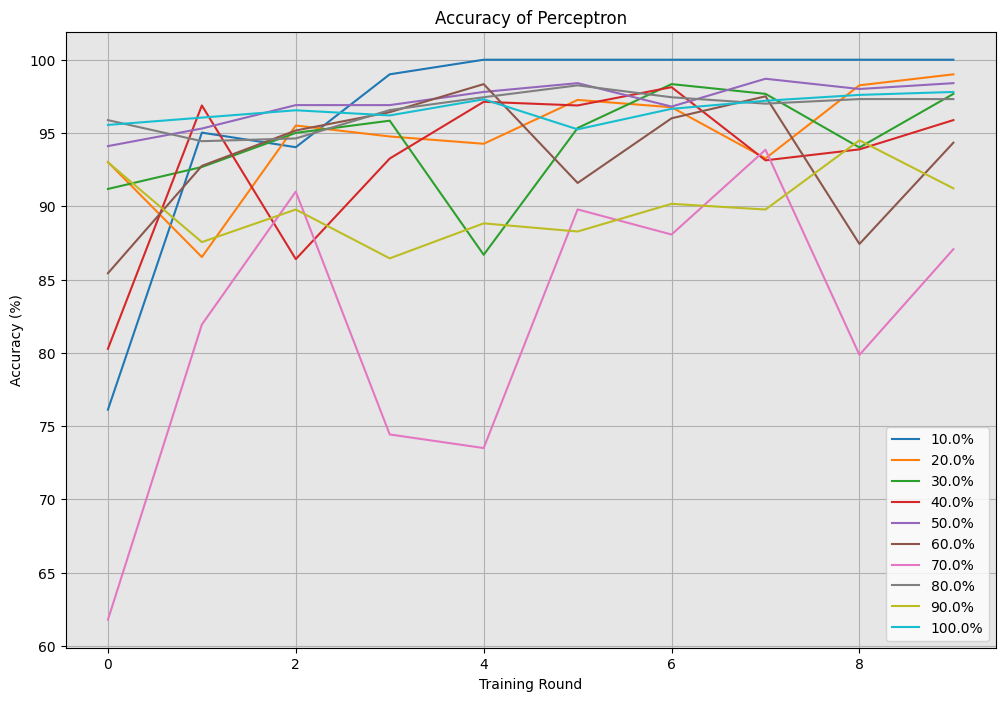
\includegraphics[width = 0.7\textwidth]{accuracy.png}
    \caption{Accuracy of the perceptron on over 10 Training Rounds. Each line represents a different percentage of the training data revealed to the perceptron. }
    \label{fig:accuracy}
\end{figure}
\end{document}